\documentclass{article}
\usepackage{graphicx} %package to manage images
\usepackage[utf8]{inputenc}
\usepackage[a4paper, total={6in, 8in}]{geometry}
\usepackage{xurl}
\title{Relatório 10 \\ Análise de transições}
\author{Pedro A. S. O. Neto}
\date{Julho, 2022}

\begin{document}

\maketitle

\section{Pupilometria}

Análise do diâmetro da pupila ao longo dos trials.

\subsection{Pre-processamento}

Normalização feita segundo a formula $(i_{t}-m)/sd$, onde $i$ representa o diâmetro da pupila no momento $t$, $m$ e $sd$ representam, respectivamente, a média e o desvio padrão do diâmetro da pupila ao longo de uma única trial.

\subsection{Análise 1 - Diâmetro da pupila em diferentes tipos de trial}

Média de pupila entre todos os participantes durante trials RJA e IJA, para vídeos com foco no brinquedo da direita e no brinquedo da esquerda. O eixo y indica a área onde a criança está olhando, enquanto a divisão dos gráficos indica o foco do trial.

Exemplo de como ler o gráfico abaixo: em média, a pupila apresenta um diâmetro menor quando a criança olha para o brinquedo da esquerda durante um trial cujo foco é o brinquedo da direita.

\begin{figure}[t]
\caption{IJA}
\noindent\makebox[\textwidth]{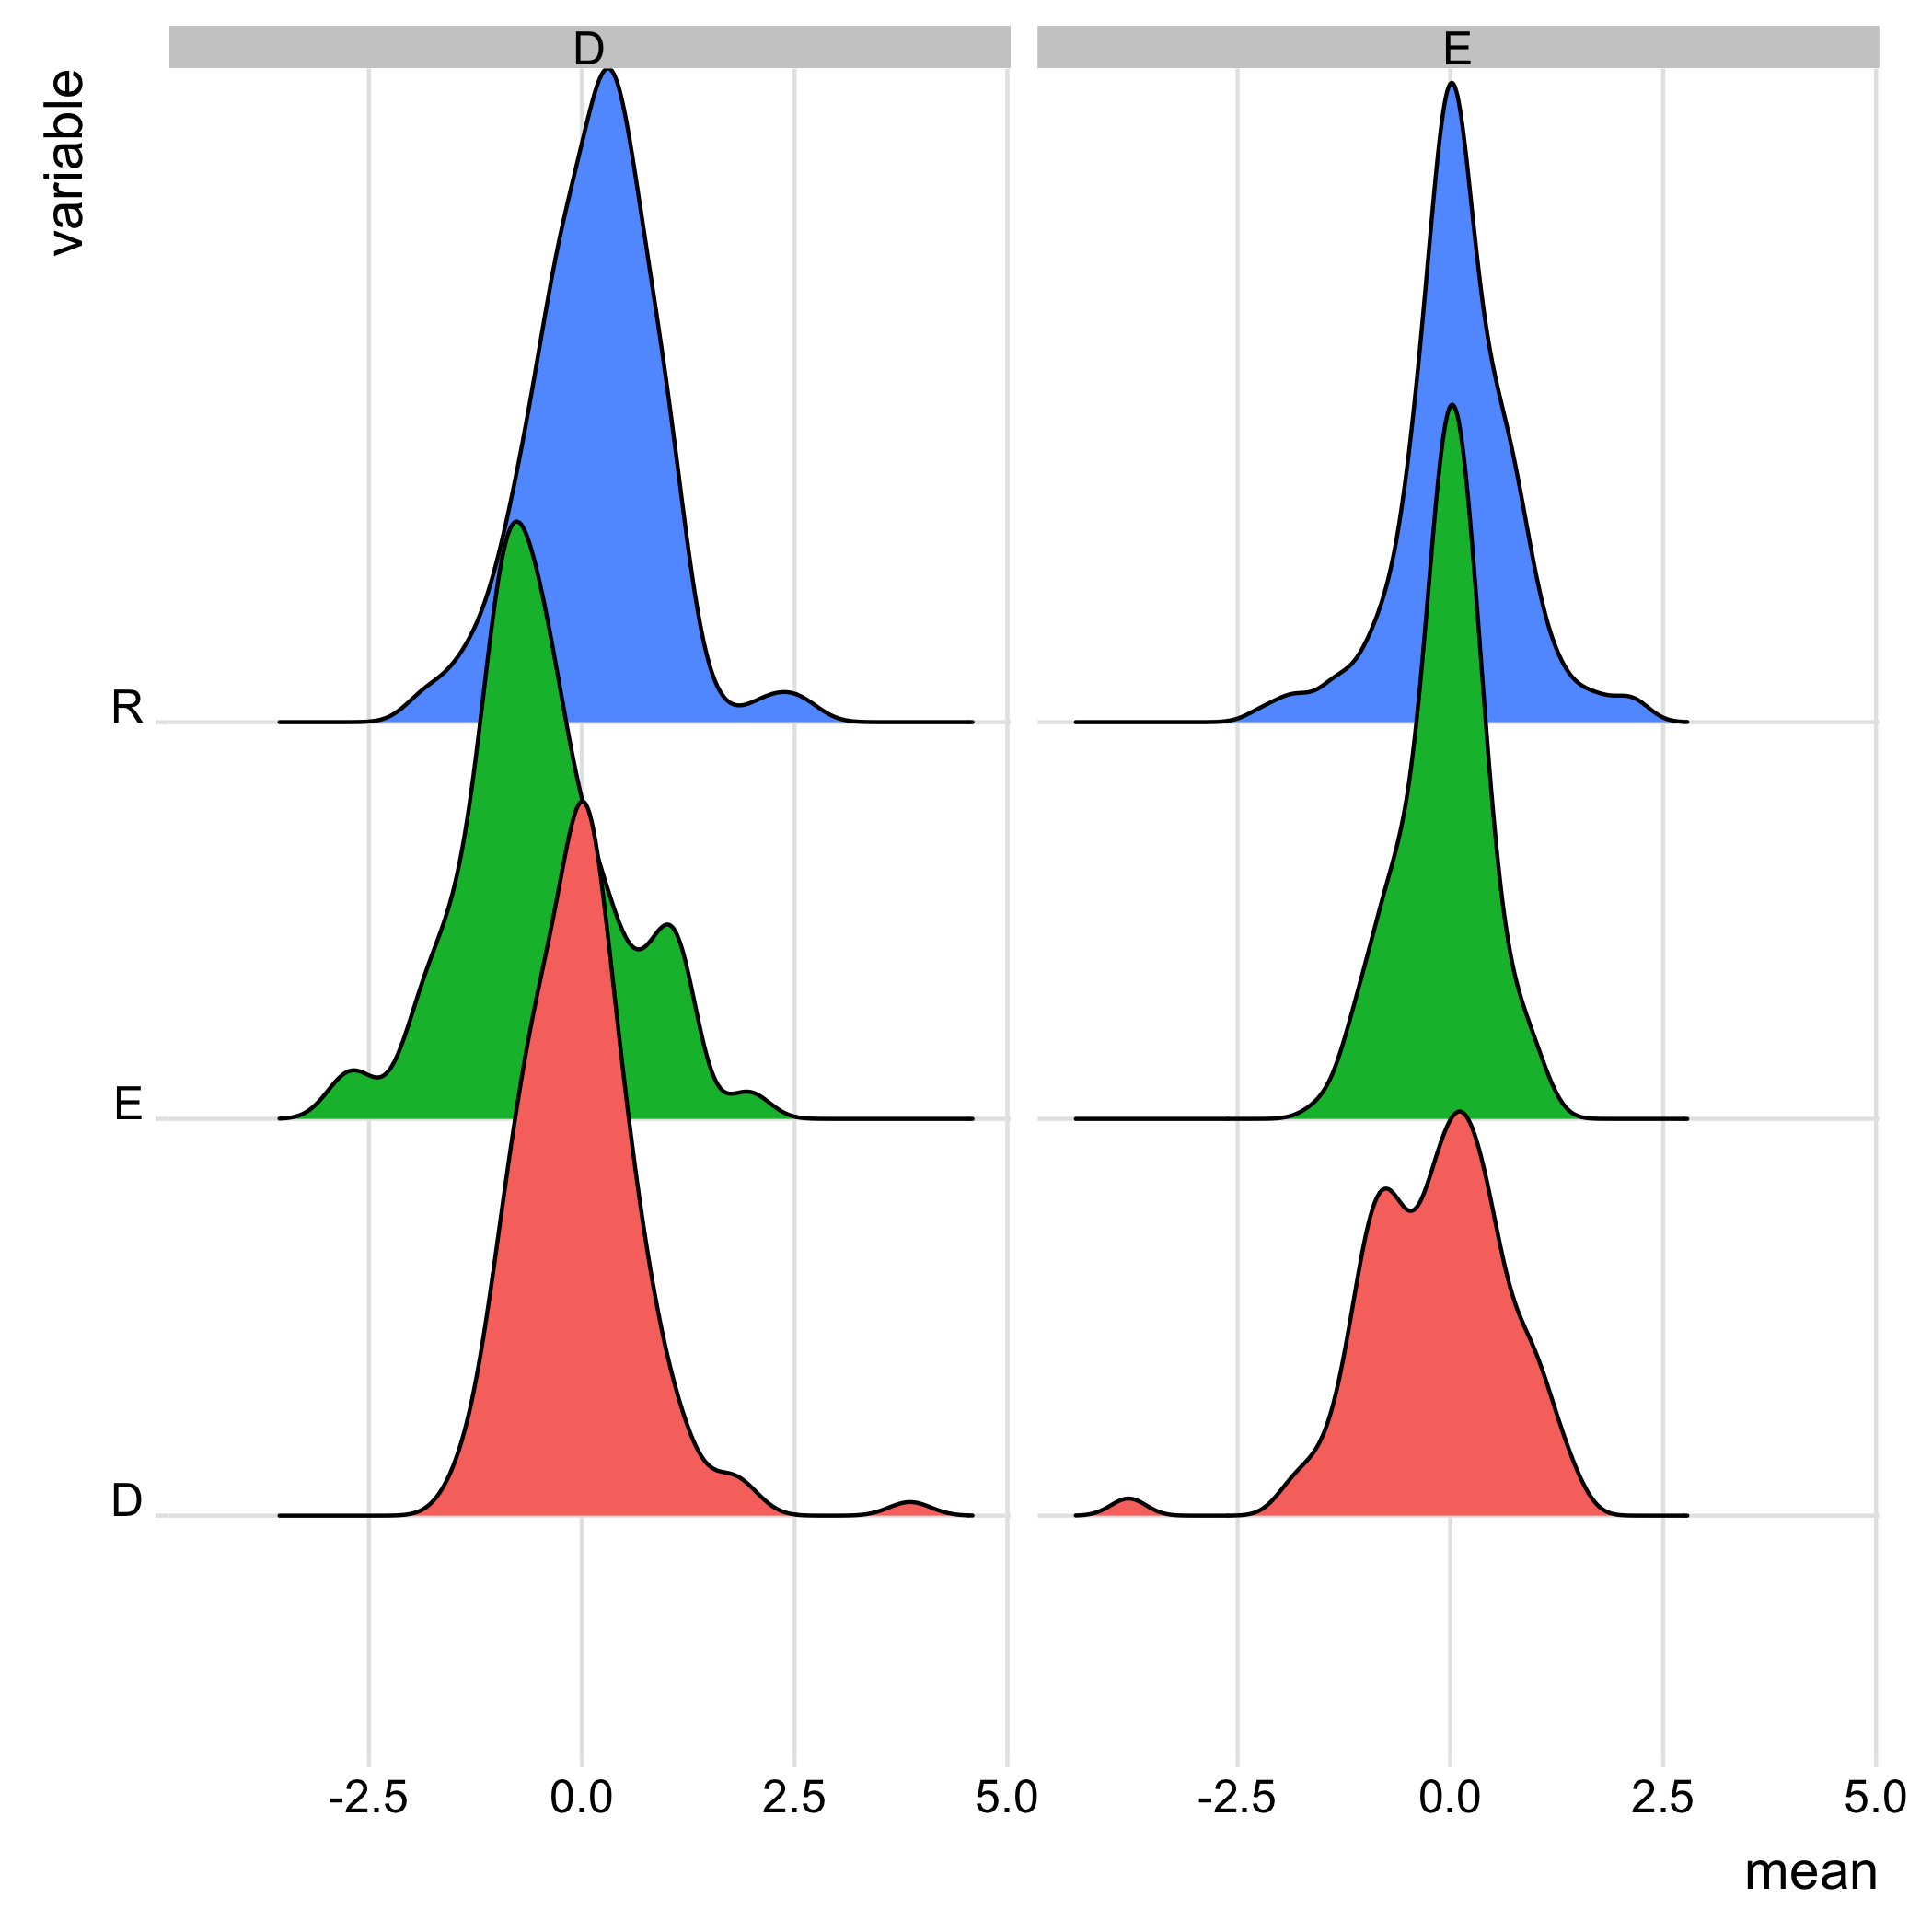
\includegraphics[scale=0.2]{"./totalIJA.png"}}
\centering
\end{figure}

\begin{figure}[t]
\caption{RJA}
\noindent\makebox[\textwidth]{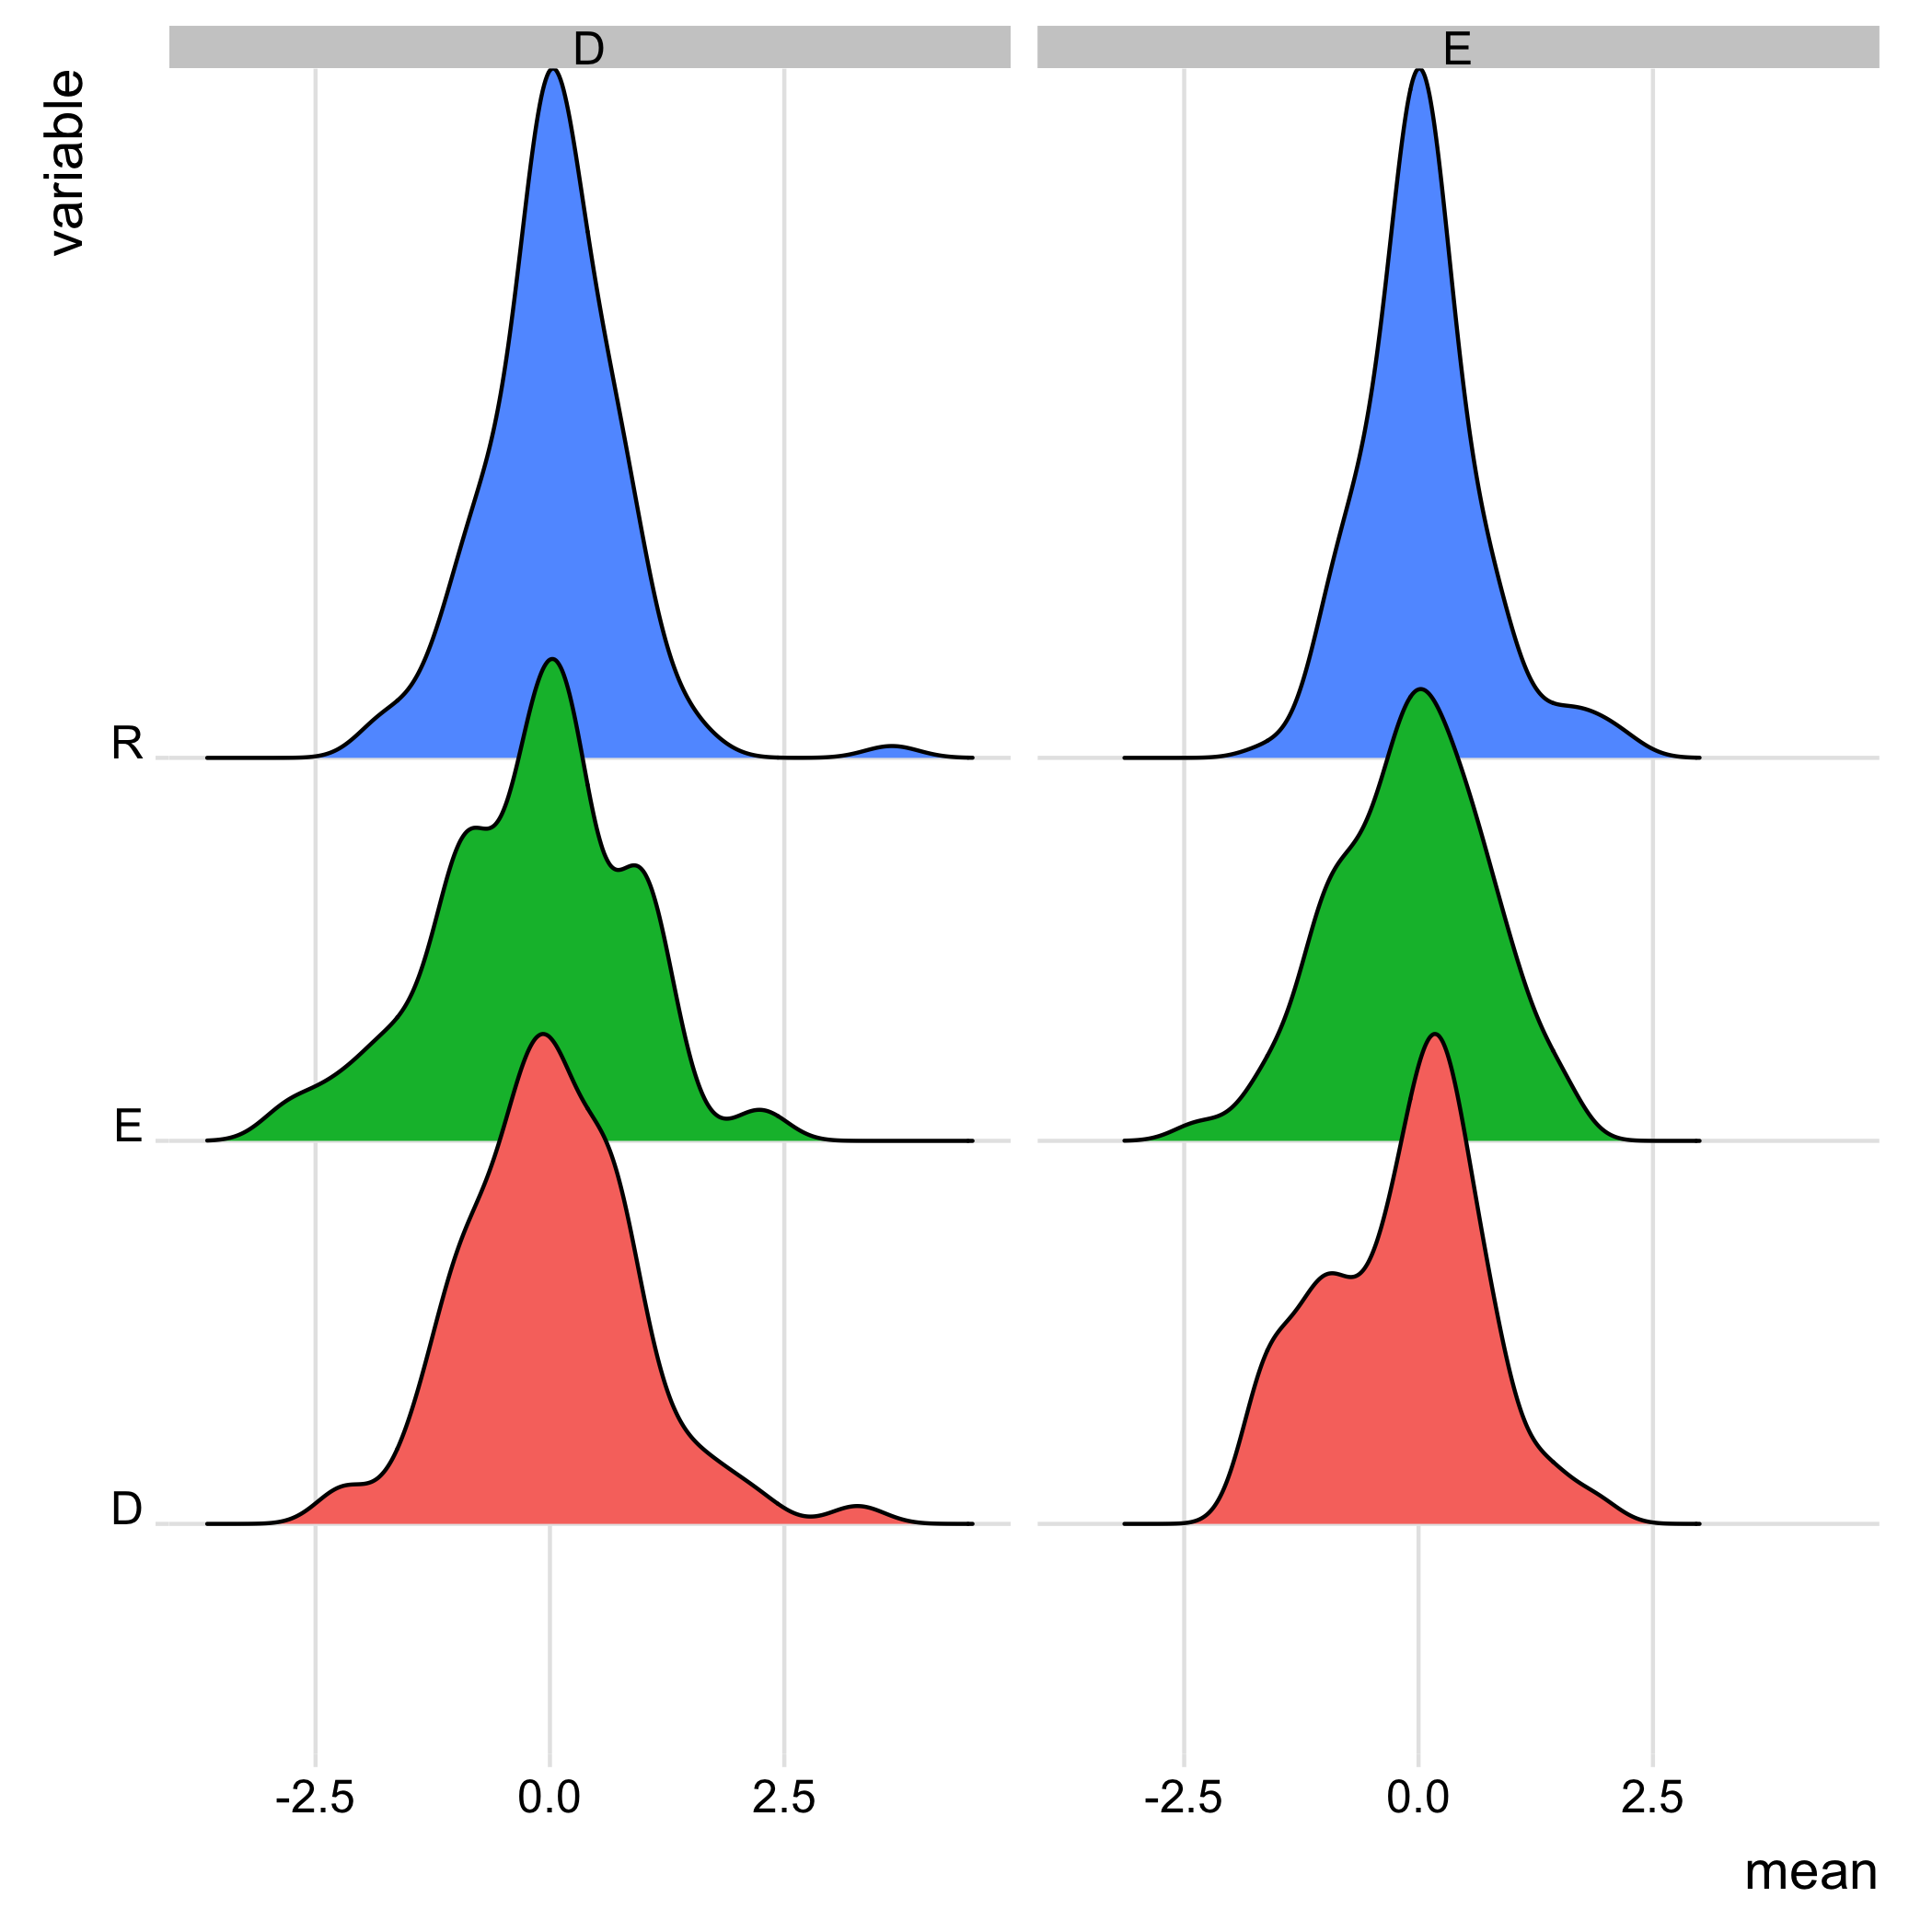
\includegraphics[scale=0.2]{"./totalRJA.png"}}
\centering
\end{figure}

\subsection{Análise 2 - Curva pupilométrica}

Análise contínua do diâmetro de pupila durante cada trial. Cores indicam qual parte da tela a criança está olhando naquele momento. Figure 3.

\begin{figure}[t]
\caption{Um participante, dividido por trial.}
\noindent\makebox[\textwidth]{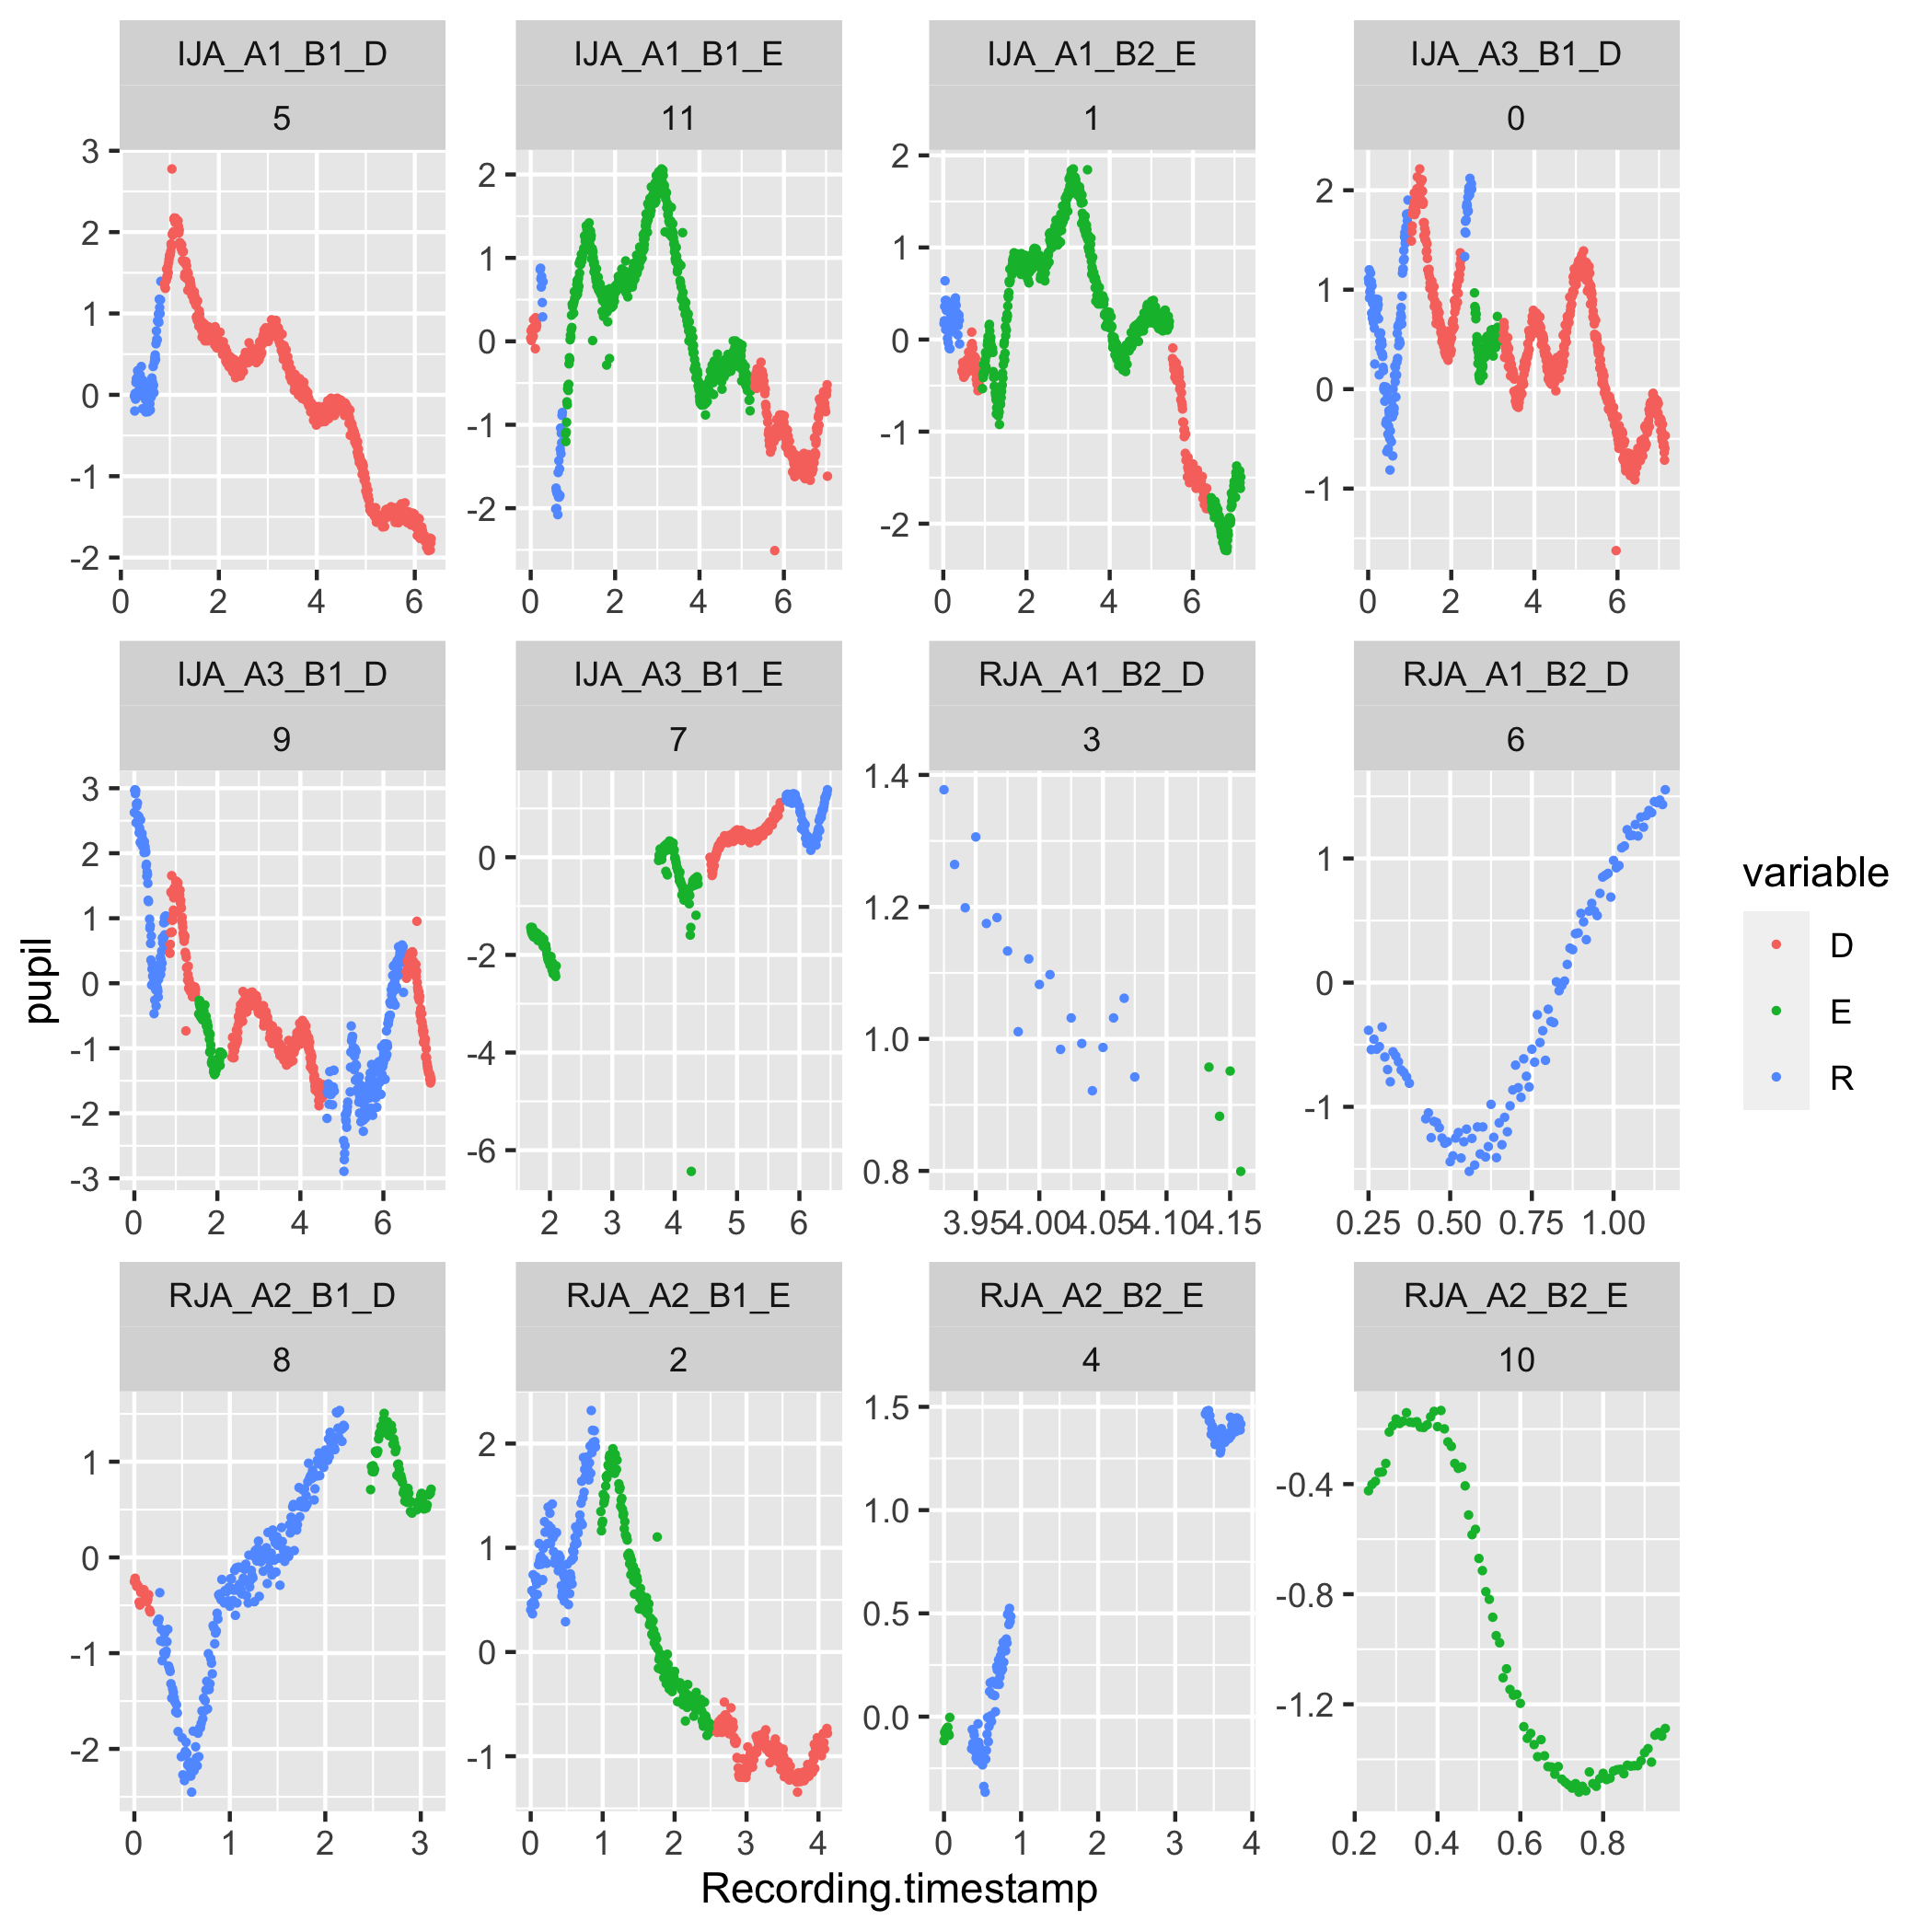
\includegraphics[scale=0.2]{"./oneParticipant.png"}}
\centering
\end{figure}

\end{document}

